%% Figure from MATH 556 notes, section 48 (Lecture 21). ADDED (not from lecture).
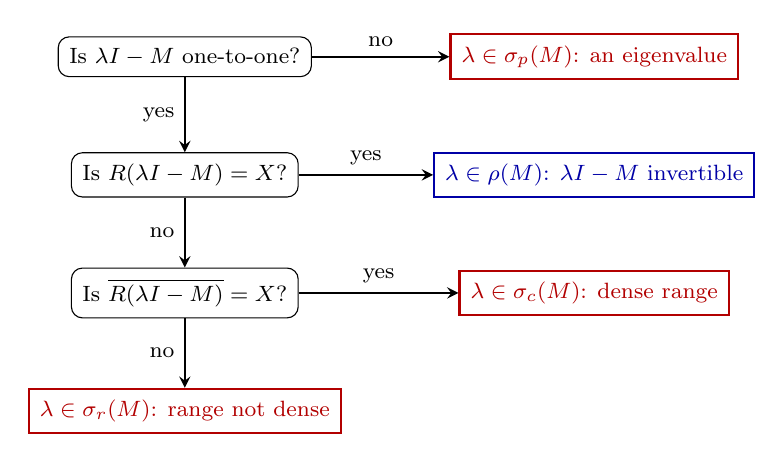
\begin{tikzpicture}[>=stealth, every node/.style={font=\footnotesize}]
    \node[draw, rounded corners, inner sep=4pt] (q1) at (0,0) {Is $\lambda I - M$ one-to-one?};
    \node[draw, rounded corners, inner sep=4pt] (q2) at (0,-1.5) {Is $R(\lambda I - M) = X$?};
    \node[draw, rounded corners, inner sep=4pt] (q3) at (0,-3.0) {Is $\overline{R(\lambda I - M)} = X$?};
    \node[draw, thick, red!70!black, inner sep=4pt] (p) at (5.2,0) {$\lambda \in \sigma_p(M)$: an eigenvalue};
    \node[draw, thick, blue!65!black, inner sep=4pt] (r) at (5.2,-1.5) {$\lambda \in \rho(M)$: $\lambda I - M$ invertible};
    \node[draw, thick, red!70!black, inner sep=4pt] (c) at (5.2,-3.0) {$\lambda \in \sigma_c(M)$: dense range};
    \node[draw, thick, red!70!black, inner sep=4pt] (s) at (0,-4.5) {$\lambda \in \sigma_r(M)$: range not dense};
    \draw[->, thick] (q1) -- node[above] {no} (p);
    \draw[->, thick] (q1) -- node[left] {yes} (q2);
    \draw[->, thick] (q2) -- node[above] {yes} (r);
    \draw[->, thick] (q2) -- node[left] {no} (q3);
    \draw[->, thick] (q3) -- node[above] {yes} (c);
    \draw[->, thick] (q3) -- node[left] {no} (s);
\end{tikzpicture}
